%%%%%%%%%%%%%%%%%%%%%%%%%%%%%%%%%%%%%%%%%%%%%%%
%%% Template for lab reports used at STIMA
%%%%%%%%%%%%%%%%%%%%%%%%%%%%%%%%%%%%%%%%%%%%%%%

%%%%%%%%%%%%%%%%%%%%%%%%%%%%%% Sets the document class for the document
% Openany is added to remove the book style of starting every new chapter on an odd page (not needed for reports)
\documentclass[10pt,english, openany]{book}

%%%%%%%%%%%%%%%%%%%%%%%%%%%%%% Loading packages that alter the style
\usepackage[]{graphicx}
% \documentclass[11pt, a4paper]{article}
\usepackage{graphicx}
\usepackage{amsmath}

\usepackage{amsmath}
\usepackage{listings}
\usepackage[]{color}
\usepackage{alltt}
\usepackage{amsmath, amssymb}
\usepackage[T1]{fontenc}
\usepackage[utf8]{inputenc}
\usepackage{lipsum}
\setcounter{secnumdepth}{3}
\setcounter{tocdepth}{3}
\setlength{\parskip}{\smallskipamount}
\setlength{\parindent}{0pt}

% Set page margins
\usepackage[top=100pt,bottom=100pt,left=68pt,right=66pt]{geometry}

% Package used for placeholder text
\usepackage{lipsum}

% Prevents LaTeX from filling out a page to the bottom
\raggedbottom

% Adding both languages
\usepackage[english]{babel}

% All page numbers positioned at the bottom of the page
\usepackage{fancyhdr}
\fancyhf{} % clear all header and footers
\fancyfoot[C]{\thepage}
\renewcommand{\headrulewidth}{0pt} % remove the header rule
\pagestyle{fancy}

% Changes the style of chapter headings
\usepackage{titlesec}
\titleformat{\chapter}
   {\normalfont\LARGE\bfseries}{\thechapter.}{1em}{}
% Change distance between chapter header and text
\titlespacing{\chapter}{0pt}{50pt}{2\baselineskip}

% Adds table captions above the table per default
\usepackage{float}
\floatstyle{plaintop}
\restylefloat{table}

% Adds space between caption and table
\usepackage[tableposition=top]{caption}

% Adds hyperlinks to references and ToC
\usepackage{hyperref}
\hypersetup{hidelinks,linkcolor = black} % Changes the link color to black and hides the hideous red border that usually is created

% If multiple images are to be added, a folder (path) with all the images can be added here 
\graphicspath{ {Figures/} }

% Separates the first part of the report/thesis in Roman numerals
\frontmatter


%%%%%%%%%%%%%%%%%%%%%%%%%%%%%% Starts the document
\begin{document}

%%% Selects the language to be used for the first couple of pages
\selectlanguage{english}

%%%%% Adds the title page
\begin{titlepage}
	\clearpage\thispagestyle{empty}
	\centering
	\vspace{1cm}

	% Titles
	% Information about the University
	{\Large Indian Institute of Technology, Madras \\ 
		Department of Electrical Engineering \\
		Applied Programming Lab \par}
		\vspace{3cm}
	{\LARGE \textbf{Lab Report}} \\
    \LARGE \textbf{Assignment 8} \\
	%\vspace{1cm}
	\vspace{3cm}
	{\large \textbf{Nithin Uppalapati} \\ 
     \large \textbf{EE18B035} \\% \\ specifies a new line
	\vspace{2cm}
    
    \centering 
\includegraphics[scale=0.2]{IITm.pdf}
%     
    \vspace{1.5cm}
		
	% Set the date
	{\normalsize 15-06-2020 \par}
	
	\pagebreak
}
\end{titlepage}

% Adds a table of contents
\tableofcontents{}

%%%%%%%%%%%%%%%%%%%%%%%%%%%%%%%%%%%%%%%%%%%%%%%%%%%%%%%%%%%%%%%%%%%%%%%%%%%%%%%%%%%%%%%%%%%%
%%%%%%%%%%%%%%%%%%%%%%%%%%%%%%%%%%%%%%%%%%%%%%%%%%%%%%%%%%%%%%%%%%%%%%%%%%%%%%%%%%%%%%%%%%%%
%%%%% Text body starts here!\\
\mainmatter

\chapter{Abstract}
Digital Signal Processing is very important as we deal with digital signals almost every single day.
\par 
For example we answer many phone calls and also take pictures from it very frequently.\\
The processing of all these signals comes under Digital Signal Processing or DSP in short.\\
\begingroup


\chapter{Introduction}

In this assignment we are going to find out DFT of various signals and plot the magnitude and phase plots.

\endgroup
% \let\clearpage\relax
\chapter{Basics of Signal Processing}
When we have a signal, observing it in time domain alone may not give us enough information. We also need the signal’s response in frequency domain.For that we have various types of transforms and series for different signals.\\
\begin{itemize}
\item Fourier Series of a signal is found out if the signal is continuous and
periodic.
\item Fourier Transform of a signal is found out if signal is continuous and
non periodic.
\end{itemize}
\begin{equation*}
f(t)=\sum_{n=-\infty}^{\infty} C_{n} e^{jnt}\\
c_{n}=\int_{to}^{to+T} f(t) e^{-jnt} dt\\
F(jw)=\int_{-\infty}^{\infty} f(t) e^{-jnt} dt\\
f(t)=\int_{-\infty}^{\infty} F(jw) e^{jnt} dt\\
\end{equation*}
\begin{itemize}
\item If f[n] is now periodic we then calculate what is known as Discrete Fourier Series or DFS of f[n] or DFT in the case N samples of a non periodic f[n] are taken and its DFS is calculated.Let period of f[n] be N then the DFT or DFS of a signal is also discrete and periodic with period N.
\end{itemize}
\begin{equation*}
F[k]=\sum{0}^{N-1} f[n] e^{-2\pi j nk/N}= 
\sum_{0}^{N-1} f[n] W^{ nk}
\end{equation*}
Since DFT is both periodic and discrete we can store its values in a computer
and process the signal.



\section{Computing DFT}
The commands used for computing DFT and inverse DFT of signal are in a module called numpy or pylab(which contains numpy). The commands are as shown below
\begin{verbatim}
numpy.fft.fft()
numpy.fft.ifft()
\end{verbatim}
We also have another command called fftshift() which essentially places zero frequency in the frequency spectrum in the center of the graph.

\section{The Assignment}

\subsection{Problem 1}
In the first problem we have to find the frequency spectrum of $ sin^{3}t$ and $cos^{3}t$.\par
We first define the number of samples that we need for the signal. The more samples we gather, the better the spectrum but takes more time.\\
For $sin^{3}t$ and $cos^{3}t$ samples are enough to identify the spectrum. \\Then we find DFT of the sampled signal and plot its magnitude and phase.



\begin{verbatim}
n=2**7
x=linspace(0,2*pi,n+1)
x=x[:-1] ;y=sin(x)**3
Y=(fftshift(fft(y))/n)
w=linspace(-64,63,n)
figure()
subplot(2,1,1)
plot(w,abs(Y),lw=2)
xlim([-10,10])
ylabel(r"$|Y|$",size=16)
title(r"Spectrum of $\sin^3(t)$") subplot(2,1,2)
plot(w,angle(Y),’ro’,lw=2)
ii=where(abs(Y)>1e-3) 
plot(w[ii],angle(Y[ii])*180/pi,’go’,lw=2) 
xlim([-10,10])
ylabel(r"Phase of $Y$",size=16) 
xlabel(r"$k$",size=16)
\end{verbatim}
We use linspace command to create samples of x at which sin3(x) is com- puted.\\
To avoid repletion of 0 and $2\pi$ both we divide x into n+1 samples and delete the last sample.\\
After plotting we limit the x axis using xlim command to observe the signal better.\\
{\centering 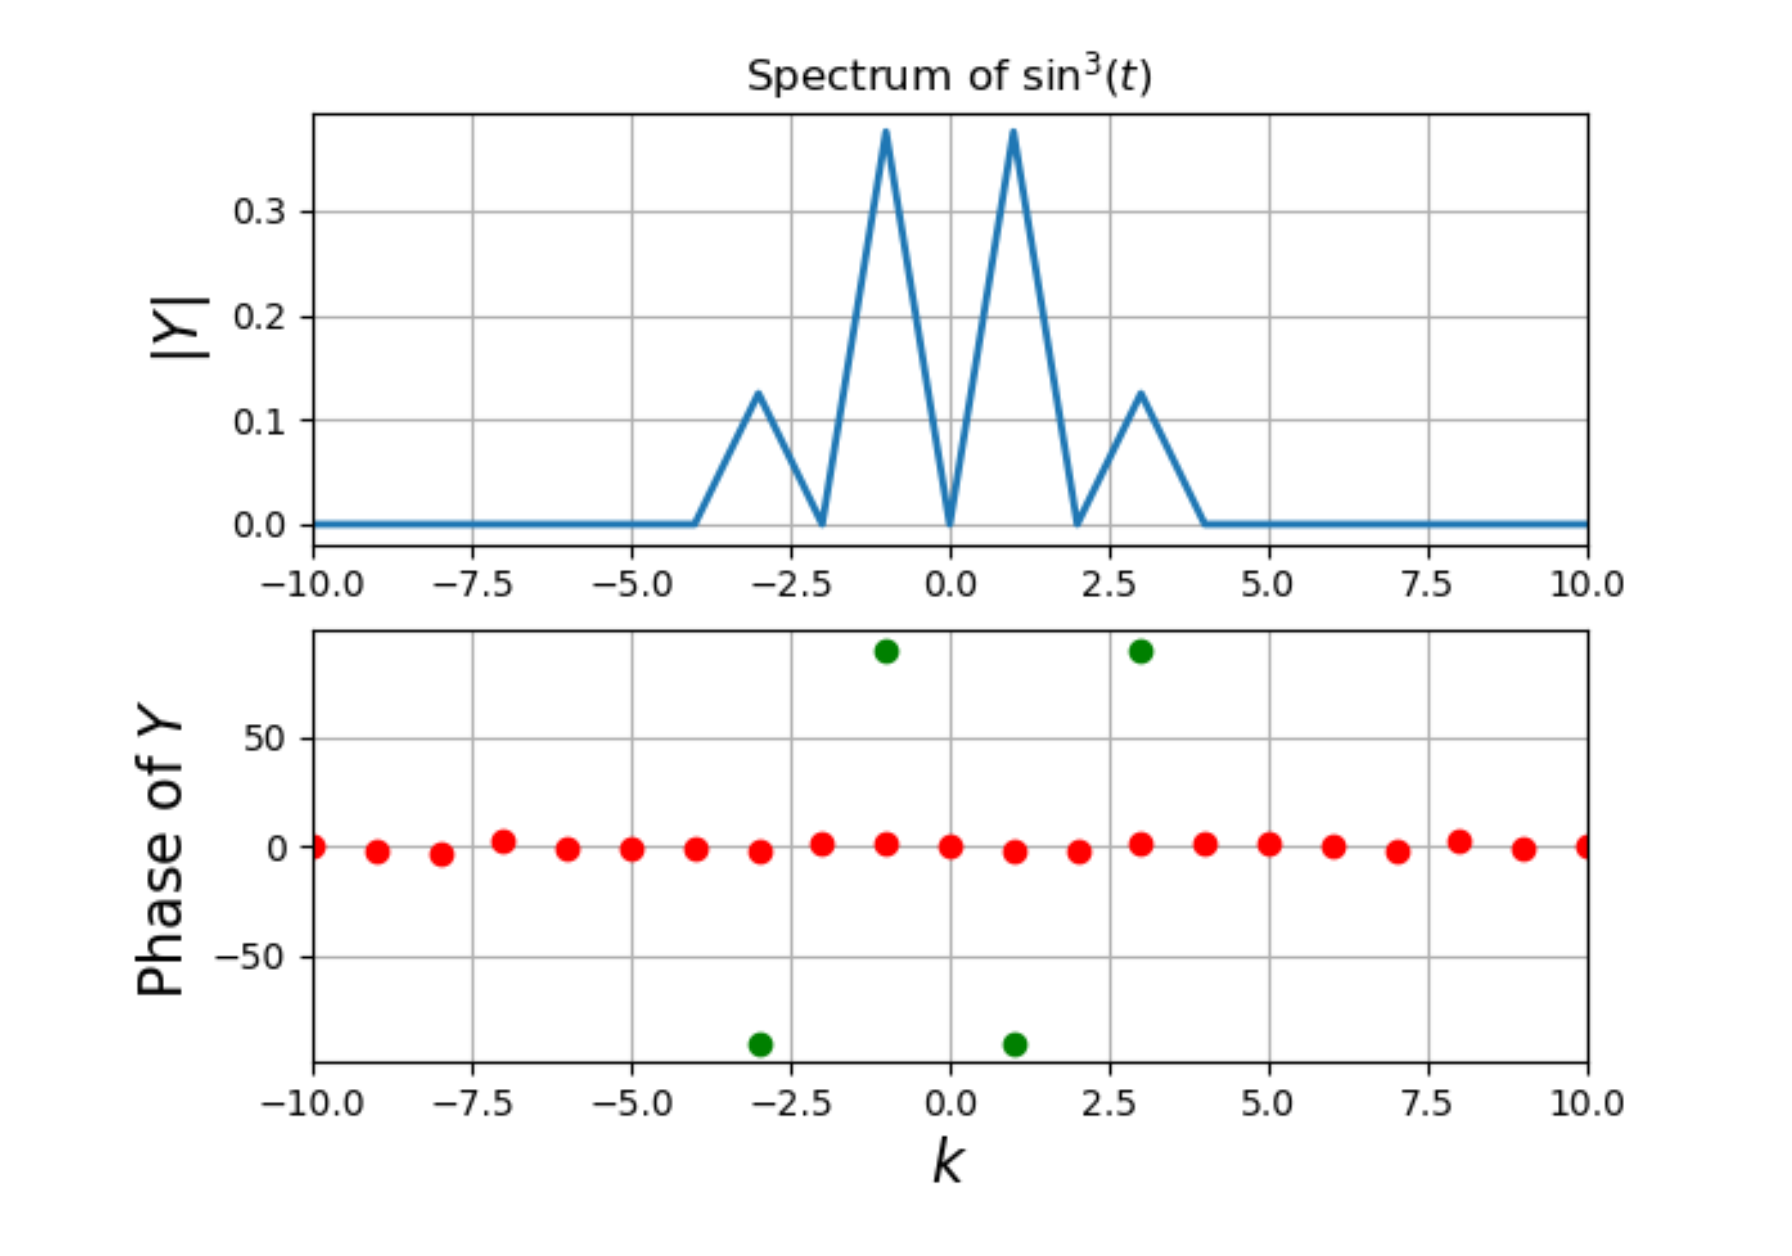
\includegraphics[scale=0.3]{Figure1.png}}\\
Similar process is done for $cos^{3}x$

\begin{verbatim}
y=cos(x)**3
Y=fftshift(fft(y))/n/2
w=linspace(-64,63,n)
figure()
subplot(2,1,1)
plot(w,abs(Y),lw=2)
xlim([-10,10])
ylabel(r"$|Y|$",size=16)
title(r"Spectrum of $\cos^3(t)$")
subplot(2,1,2)
plot(w,angle(Y)*180/pi,'ro',lw=2)
ii=where(abs(Y)>1e-3)
plot(w[ii],angle(Y[ii])*180/pi,'go',lw=2)
xlim([-10,10])
ylabel(r"Phase of $Y$",size=16)
xlabel(r"$k$",size=16)
\end{verbatim}
If we plot phase of DFT at all points we get a messed up graph. So we compute phase for points at which magnitude is greater than 0.001.

{\centering 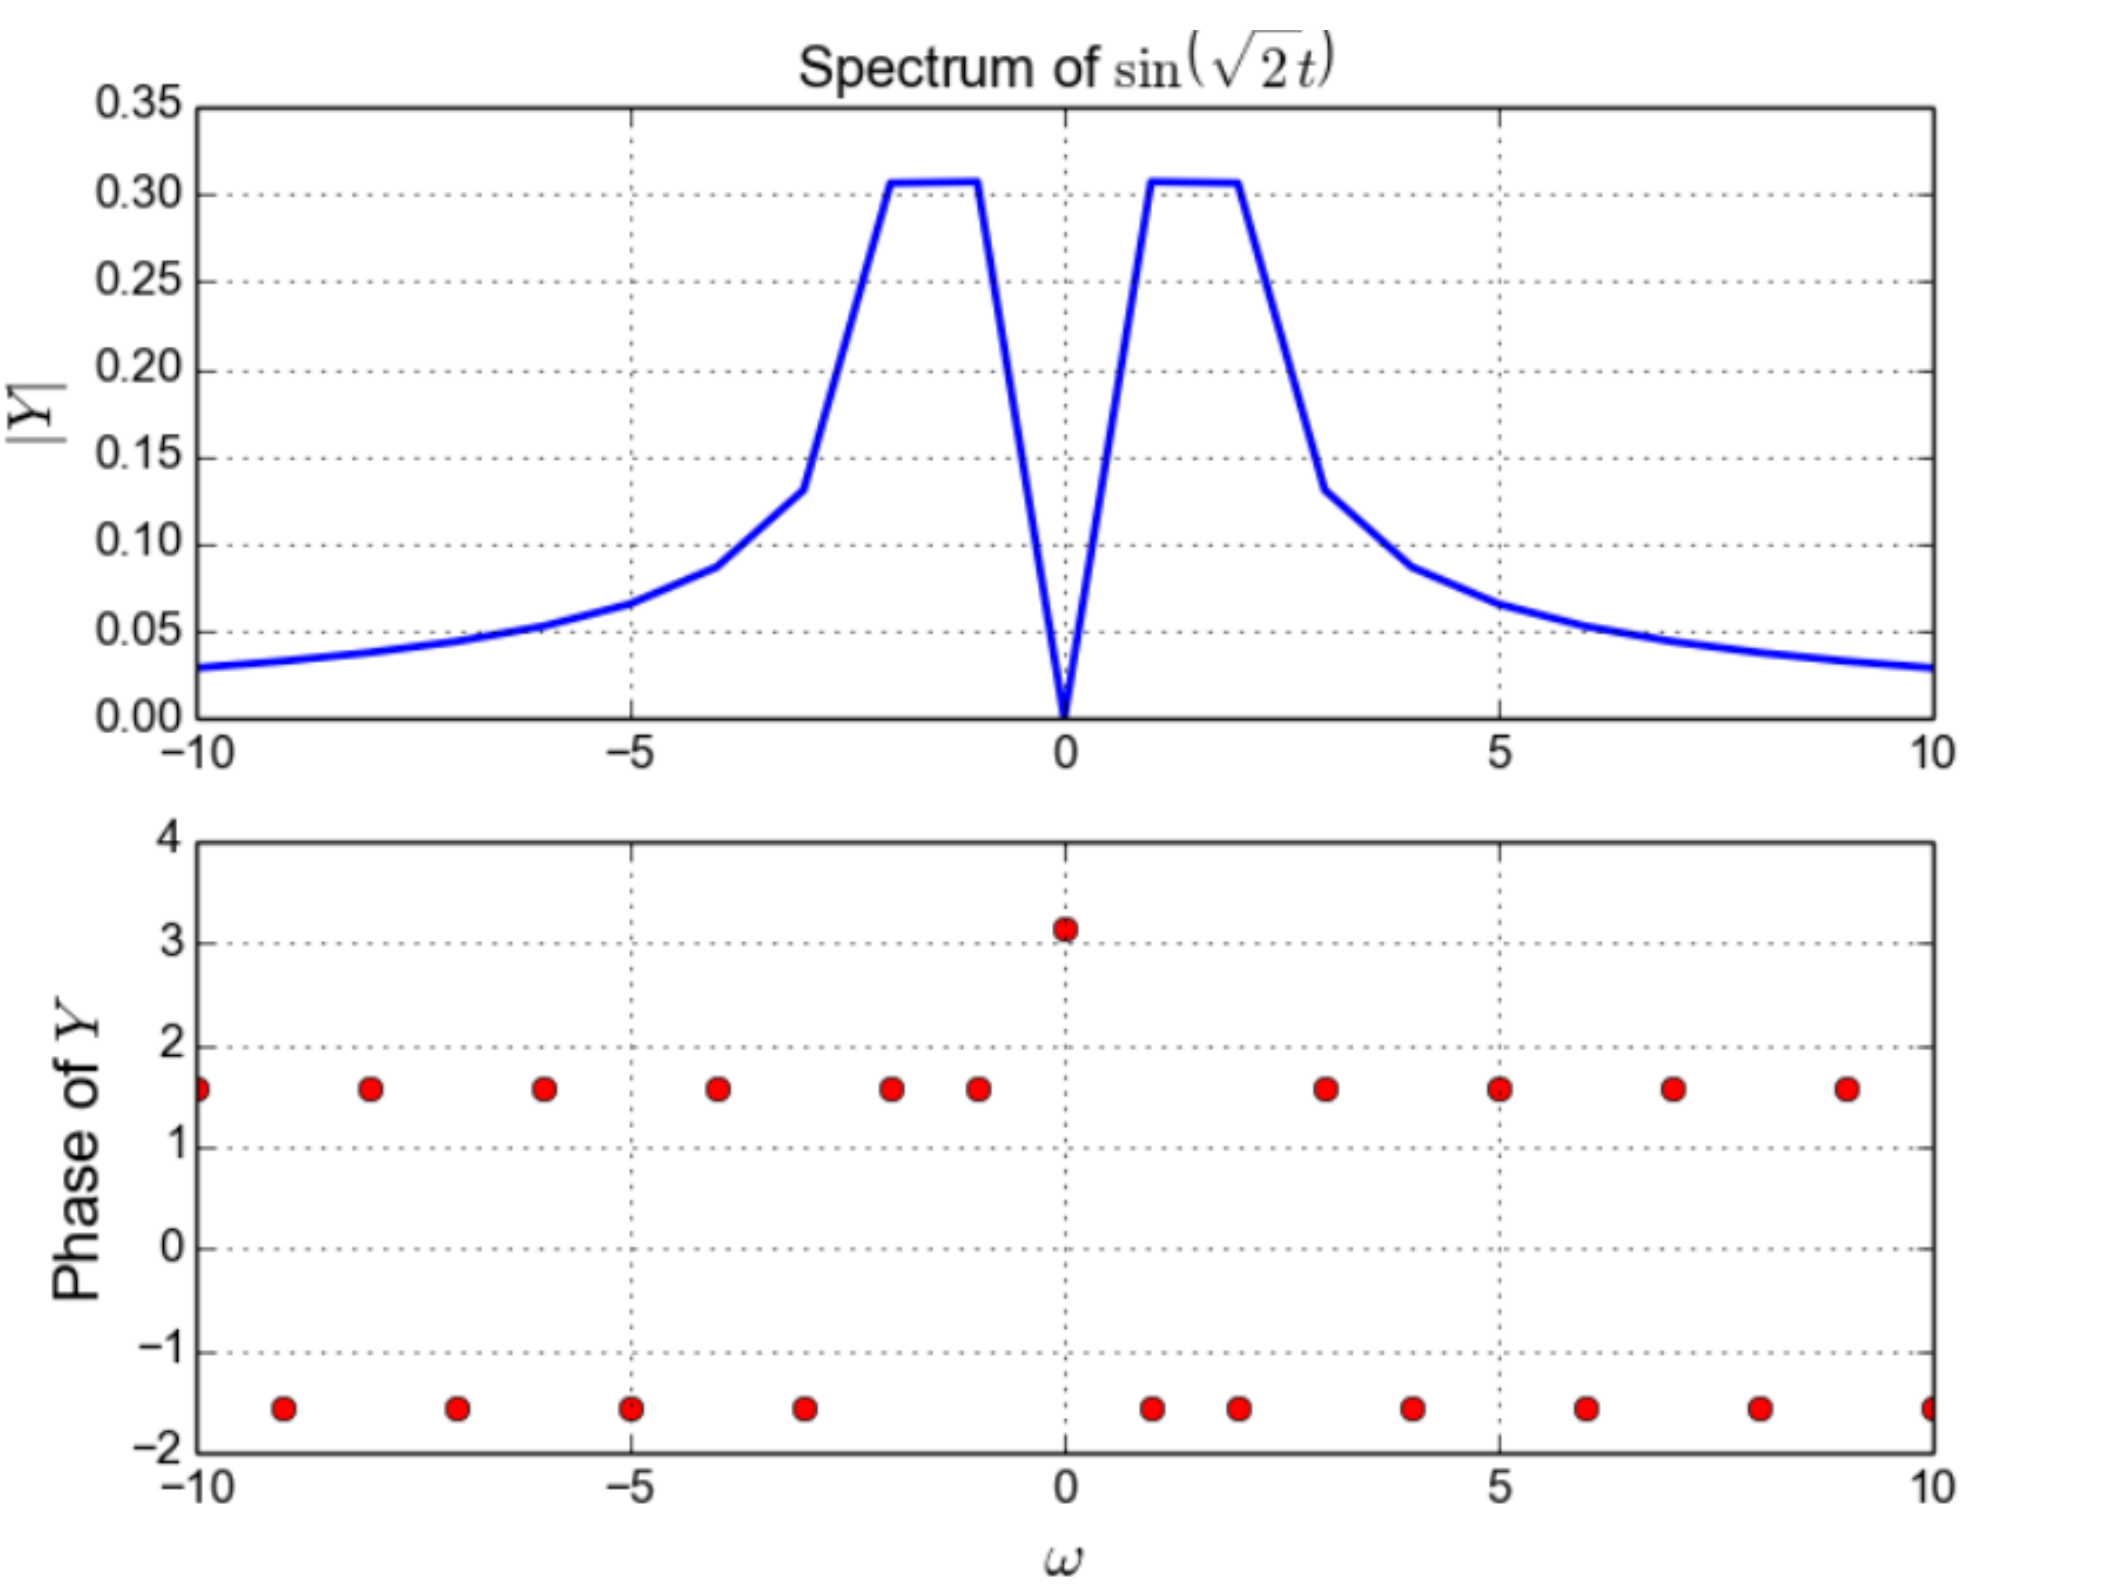
\includegraphics[scale=0.3]{Figure2.png}}

\subsection{Problem 2}

In this problem we have to find DFT of $ cos(20 + 5cos(x))$ .Compared to $sin^{3}(x)$ this signal has a wider frequency band and peaks in magnitude closer to each other. So we need slightly higher samples for computation.We use $2^{10}$ samples.//

\begin{verbatim}
n=2**10
x=linspace(-2*pi,2*pi,n+1);x=x[:-1]
y=cos(20*x+5*cos(x))
Y=fftshift(fft(y)/n)*2
\end{verbatim}

In this case we divided x from $ -10\pi$ to $10\pi$ instead of 0 to $ 2\pi$ because we need a wider spectrum to observe the peaks easily and also higher samples to distinguish between the peaks.\\

\begin{verbatim}
w=linspace(-64,64,n+1);w=w[:-1]
figure()
subplot(2,1,1)
plot(w,abs(Y),lw=2)
xlim([-60,60])
ylabel(r"$|Y|$",size=16)
title(r"Spectrum of $\cos(20x+5\cos(x))$") 
subplot(2,1,2)
ii=where(abs(Y)>1e-3) 
plot(w[ii],angle(Y[ii])*180/pi,color=’orange’,lw=2) 
xlim([-60,60])
ylabel(r"Phase of $Y$",size=16) xlabel(r"$k$",size=16)
\end{verbatim}
{\centering 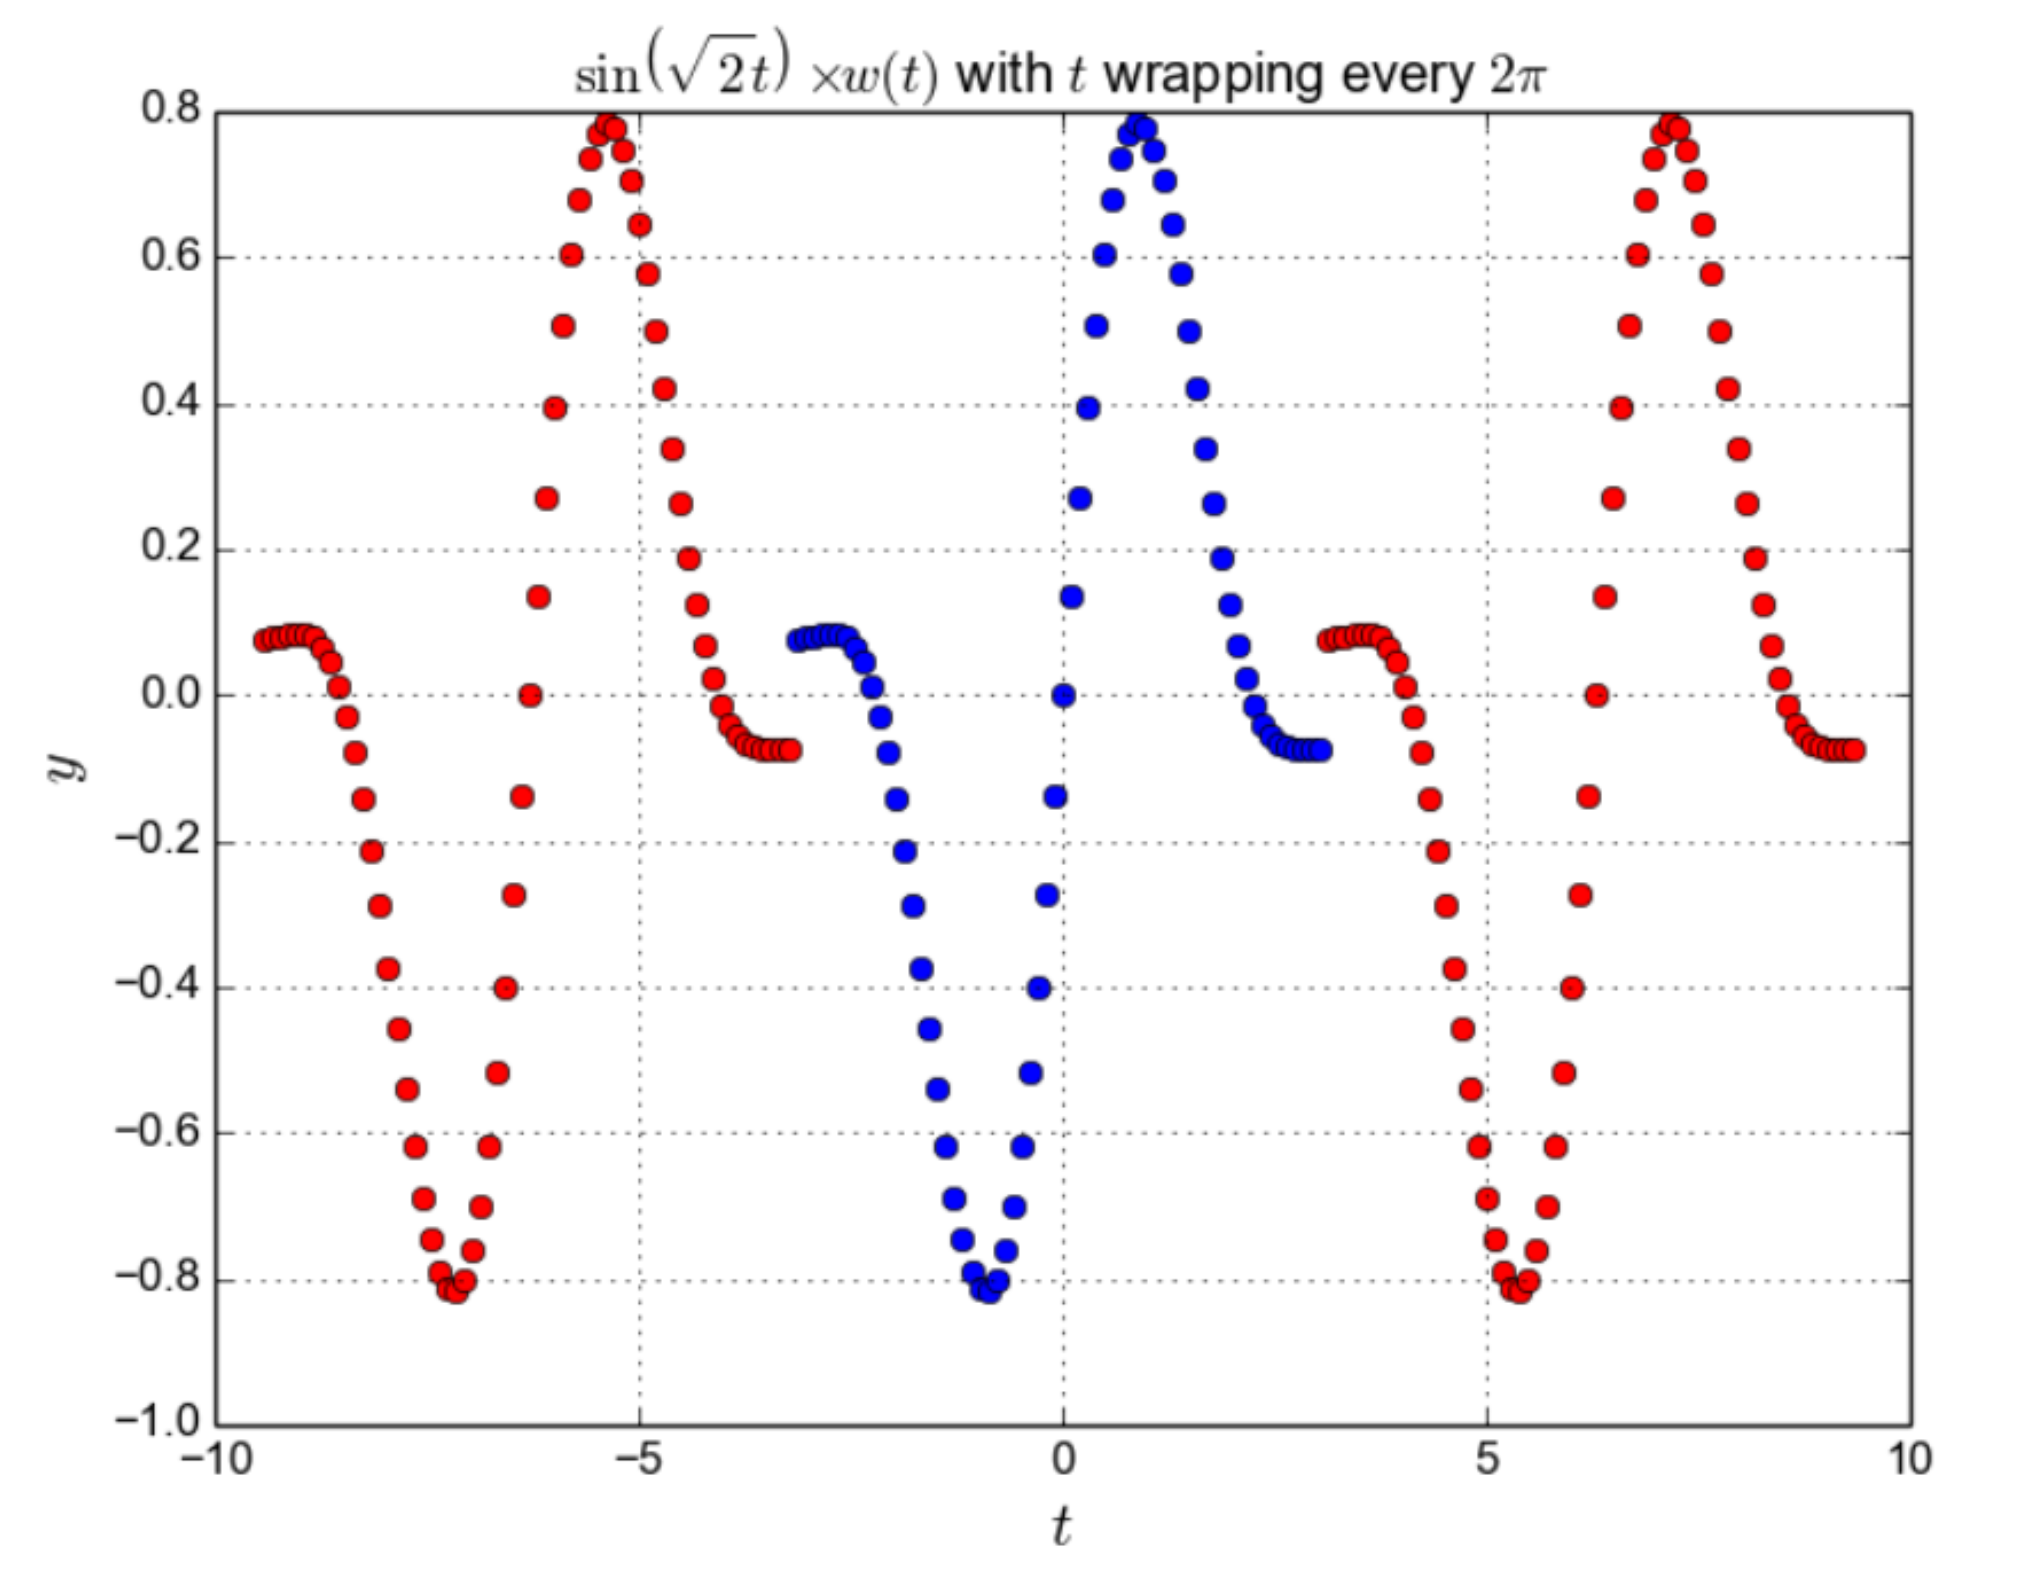
\includegraphics[scale=0.3]{Figure3.png}}



\subsection{Problem 3}

In the final problem we have to find the spectrum of$ exp(-x^{2}/2 )$.This type
of function is classified as Gaussian function and is not band-limited in frequency.\\
To get highly accurate(to 6 digits) magnitude of DFT of signal we have to take a large amount of samples.So we take 218 samples from $-8\pi $ to $8\pi$.\\

\begin{verbatim}
n=2**18
x=linspace(-8*pi,8*pi,n+1);x=x[:-1]
y=exp(-x**2/2)
Y=(fftshift(fft(y))/n)*8 
w=linspace(-n/2,n/2,n+1);w=w[:-1]
figure()
subplot(2,1,1)
plot(w,abs(Y),lw=2)
xlim([-30,30])
ylabel(r"$|Y|$",size=16)
title(r"Spectrum of $e(-x^2/2)$")
subplot(2,1,2)
ii=where(abs(Y)>1e-3) 
plot(w[ii],angle(Y[ii])*180/pi,color=’hotpink’,lw=2) 
xlim([-30,30])
ylabel(r"Phase of $Y$",size=16) 
xlabel(r"$k$",size=16)
\end{verbatim}


We take frequency axis from $-2^{19}$ to $ 2^{19}$ and limit the axis to length 30 on either side of 0.

{\centering 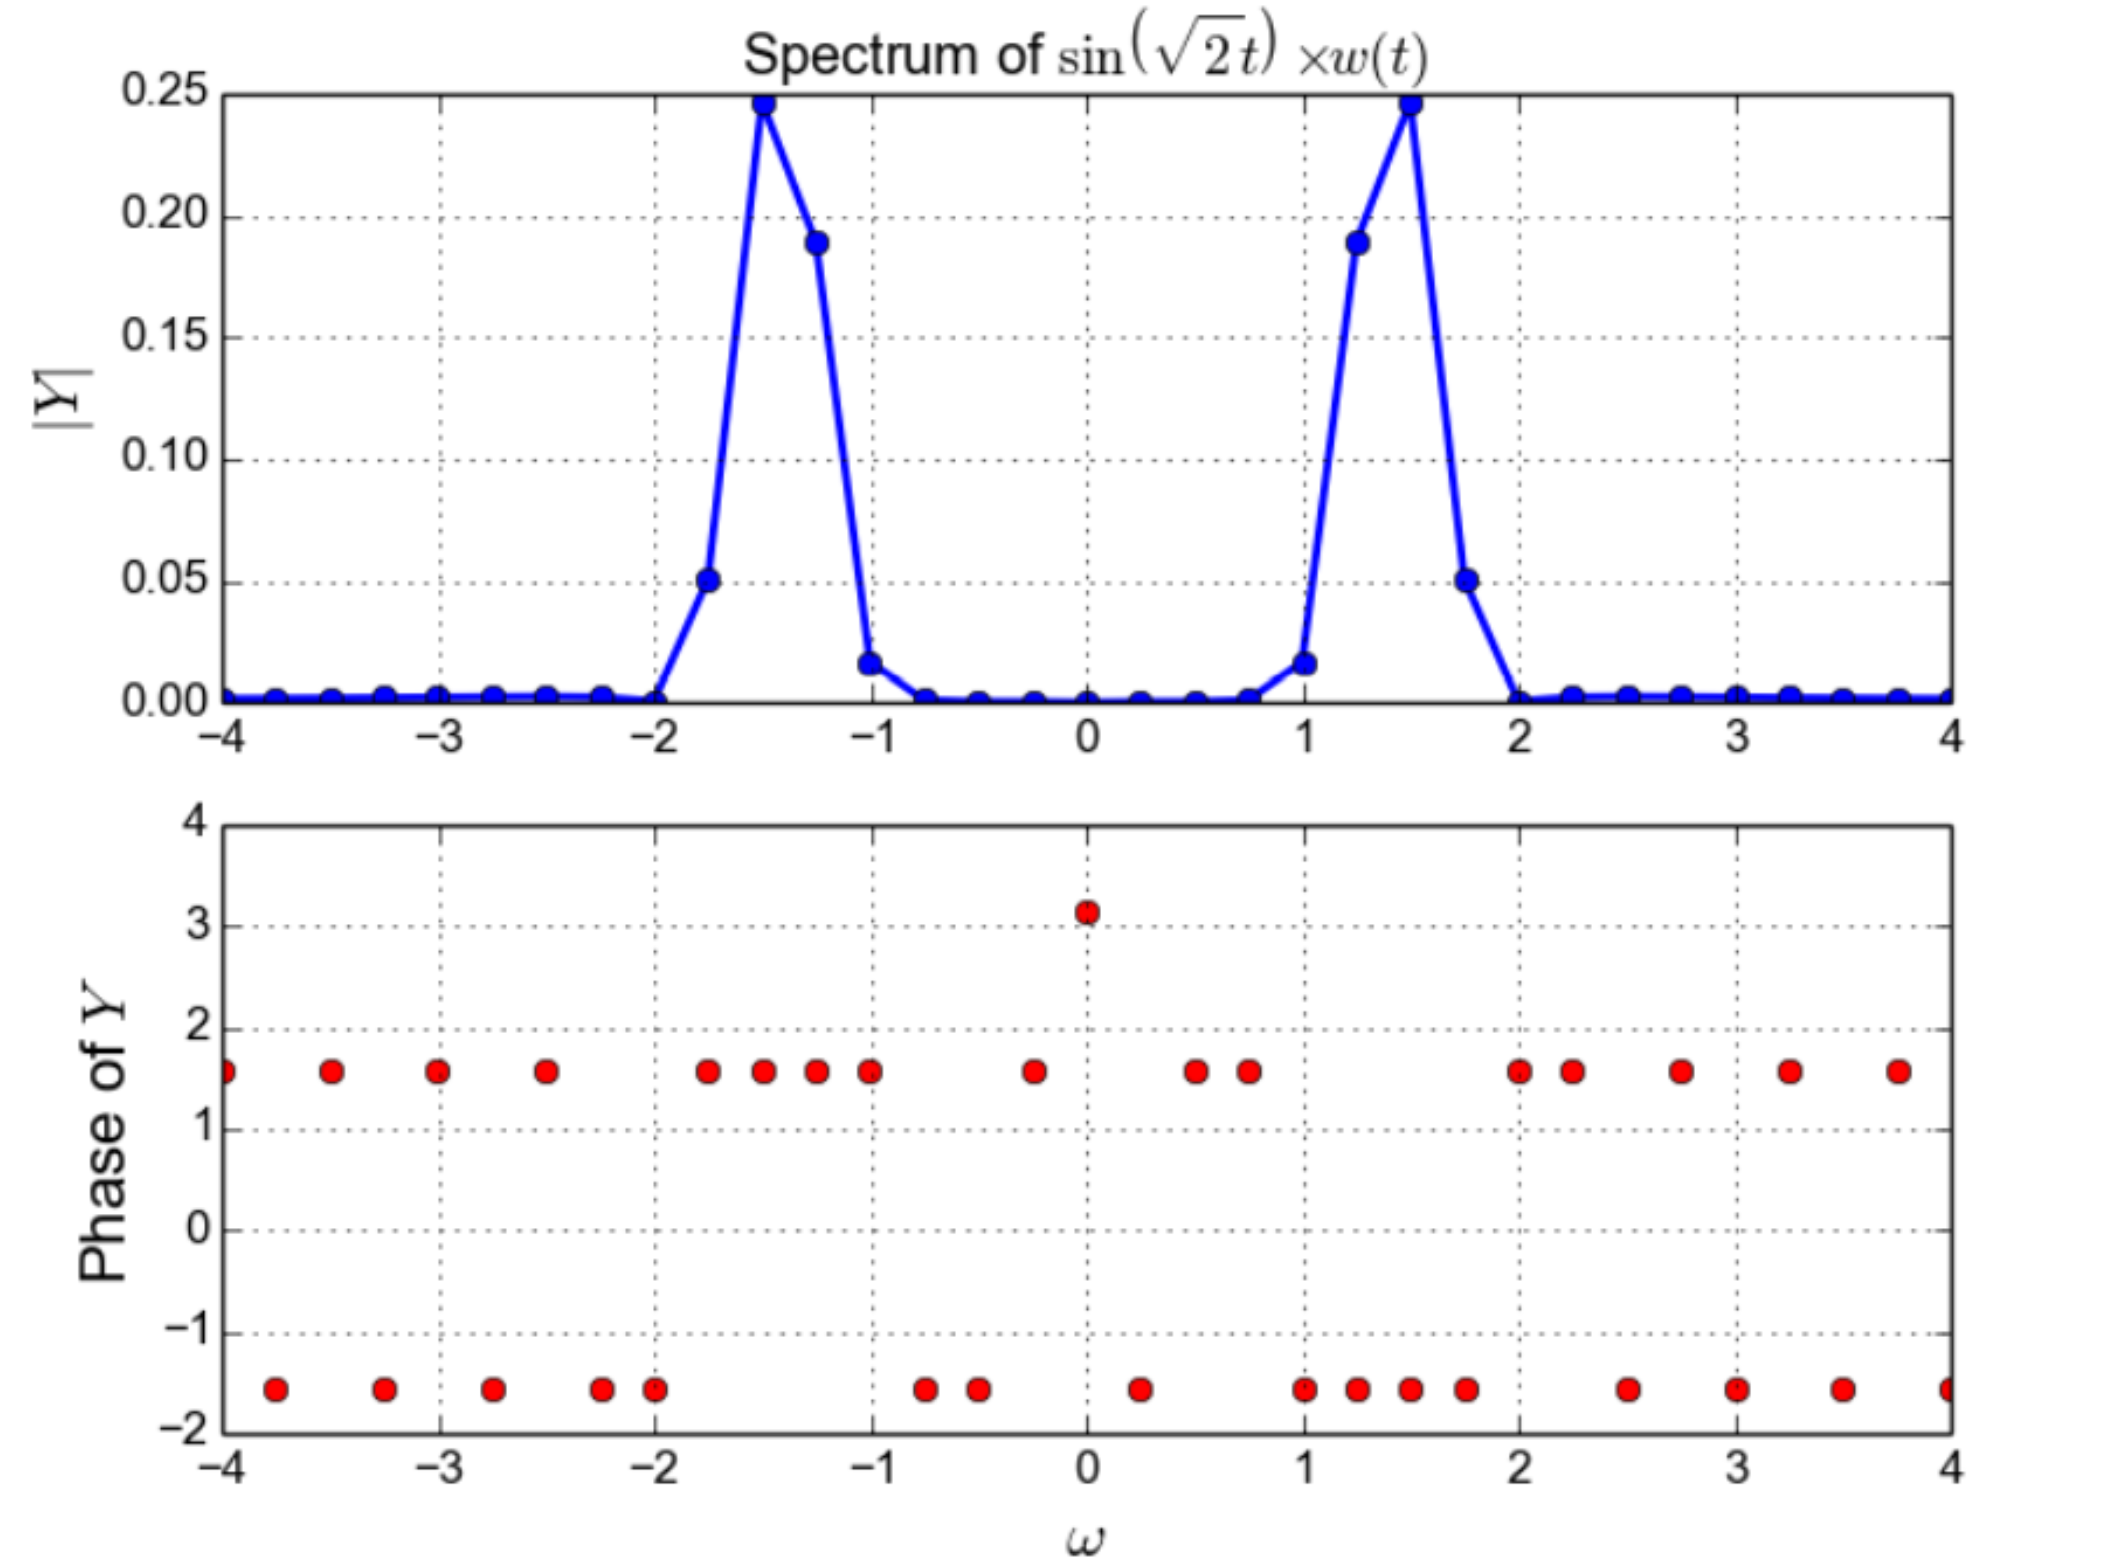
\includegraphics[scale=0.3]{Figure4.png}}\\

In this plot we can observe that the points are represented up to 6 significant digits.

\section{Observations}
Computing DFT of signals is very easy using these commands. However we have to be careful with the sampling and defining the frequency axis as things can get messy and the plots obtained may not be accurate. We also have to worry about under-sampling as we may not be able to observe distinct peaks in the frequency spectrum. The phase spectrum of the signals may not be accurate and so we should consider phase only near the peaks.

\end{document}











